%!TEX encoding=UTF-8 Unicode
%!TEX root=../tabarnac.tex

\section{TABARNAC}
\label{sec:design}

\TABARNAC is divided into two parts: the instrumentation tool and the
visualization. In this section, we discuss the implementation of both parts.

\subsection{Data collection}
\label{sec:design-impl}

\TABARNAC data collection aims at providing information on how data structure
are accessed, therefore, it needs to collect fine grain information. To do so,
we instrument memory access and collect the number of access per page, thread
and type (Read/Write). The information is stored on a per-thread basis, as
shown in Listing~\ref{lst:mem}, making the code completely lock-free, as well
as minimizing the amount of false sharing between threads.

\begin{lstlisting}[caption={Code executed on each memory access. The \texttt{address}, \texttt{threadid} and \texttt{type} parameters are provided by Pin.},label=lst:mem]
	void mem_access(unsigned long address, int threadid, char type){
		uint64_t page = address >> page_bits;
		acc[threadid][page][type]++;
	}
\end{lstlisting}

The instrumentation uses the Pin dynamic binary instrumentation
tool~\cite{Luk05Pin}, although it is an Intel technology, it works also on AMD
processors.

Before running the application, our tool retrieves static memory allocation
information %using the \texttt{libelfg0} library.
Dynamic allocations are intercepted with at the runtime and structure names
are extracted using the debug flags.
%\texttt{malloc} replacement. If the application is
%compiled with debug flags (\texttt{-g}), the structure names that are malloced can be extracted from the source
%code.
Finally, each time a thread is created, we compute
stack bounds, and create a virtual structure named \texttt{Stack\#N} where
$N$ is the thread id. Only structures that are bigger than one page (usually
$4$Kib in current x86\_64 architectures) are recorded as our
analysis granularity is the memory page. The data structure informations (name,
size and address) are only used to generate the visualization, after the end
of the instrumentation.

%For each access, we store the type (read or write), the memory page that was
%accessed, and the thread ID responsible of it.
%\caption{Code that is executed on each memory access.}
%\label{fig:code}
%\end{figure}


%After tracing finishes, %we generate three \texttt{csv} files.  The first
%contains the list of pages and the number of reads and writes per thread. The
%second contains the list of structures with their names, sizes and start
%addresses, the last file contains the stacks size and addresses.  Then, a
%a script which reads the trace, retrieves the page / data structure mapping
%and generates the final visualization presented in the next subsection.

% not relevant I'd say:
% \TABARNAC have very few dependencies and can be installed easily. If all the R
% library required to generate the visualization are not present, our tool is
% able to install them automatically. By default \TABARNAC generate the memory
% trace and the visualization, but the user can also choose to only generate the
% memory trace or the visualization. This is useful for people who cannot
% install R on the machine used to generate the trace. Moreover it allows the
% user to customize the plots generate by the R script.

\subsection{Visualization}
\label{sec:design-visu}


Once the analysis phase is done,
\TABARNAC generates the visualization (as an HTML page), providing a summary
of the trace through several plots\footnote{A full example is available at
    \url{http://dbeniamine.github.io/Tabarnac/example}}.
The visualization aims at showing \emph{why} performances issues related
to memory occurs, it therefore shows several plots helping to understand the
importance of each data structure and how it is accessed.
For newcomers, each plot is introduced by an explanation
of its presentation, what common issues it can help to understand and provides
suggestions on how to fix these issues.  The visualization starts with a small
introduction, summarizing the main principles while developing for NUMA
machines, and shows the hardware topology of the analyzed machine extracted
with Hwloc~\cite{Broquedis10hwloc}.

\begin{figure*}[h!]
    \centering
    \subfigure[Structures size.]{
        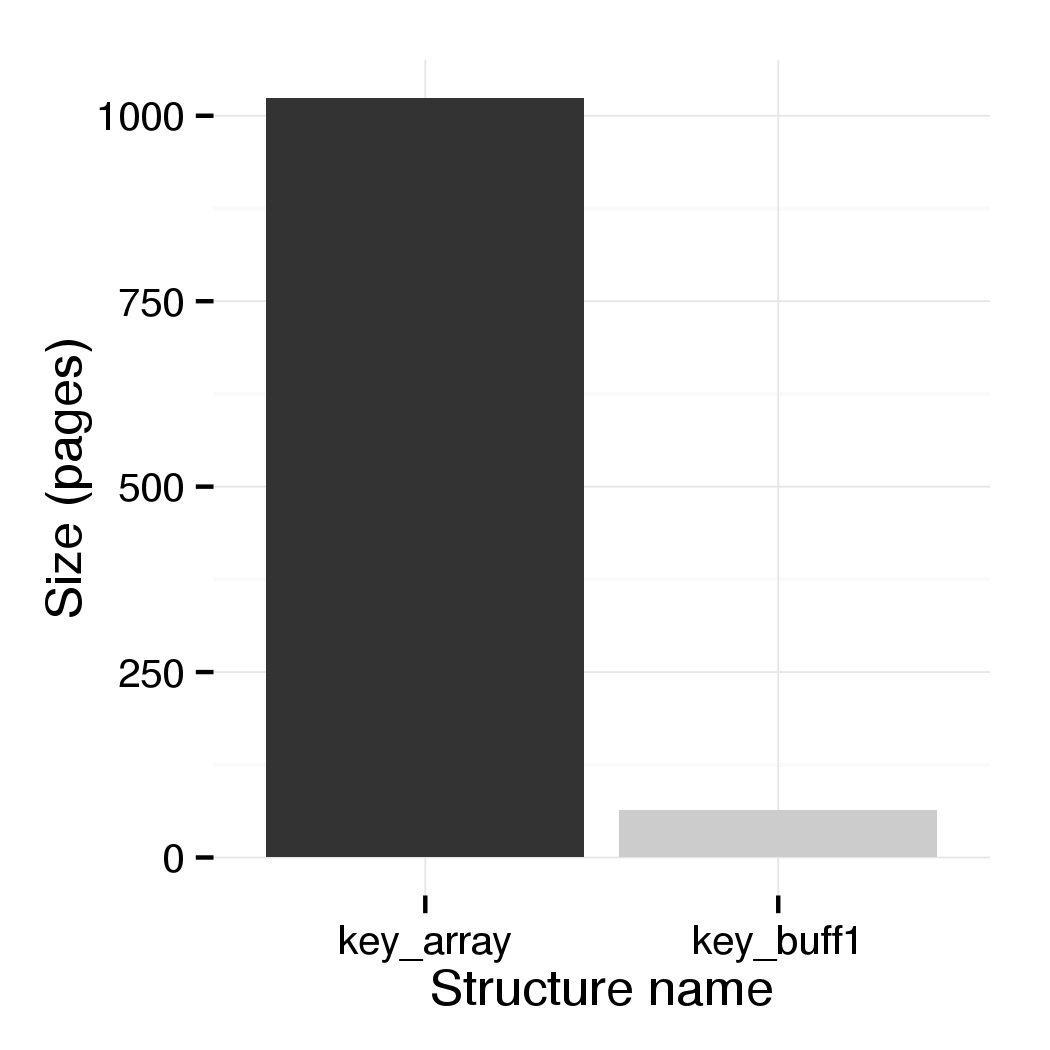
\includegraphics[height=.2\textheight]{example_sz}
        \label{fig:example_sz}
    }
    \subfigure[Number of accesses per structures.]{
        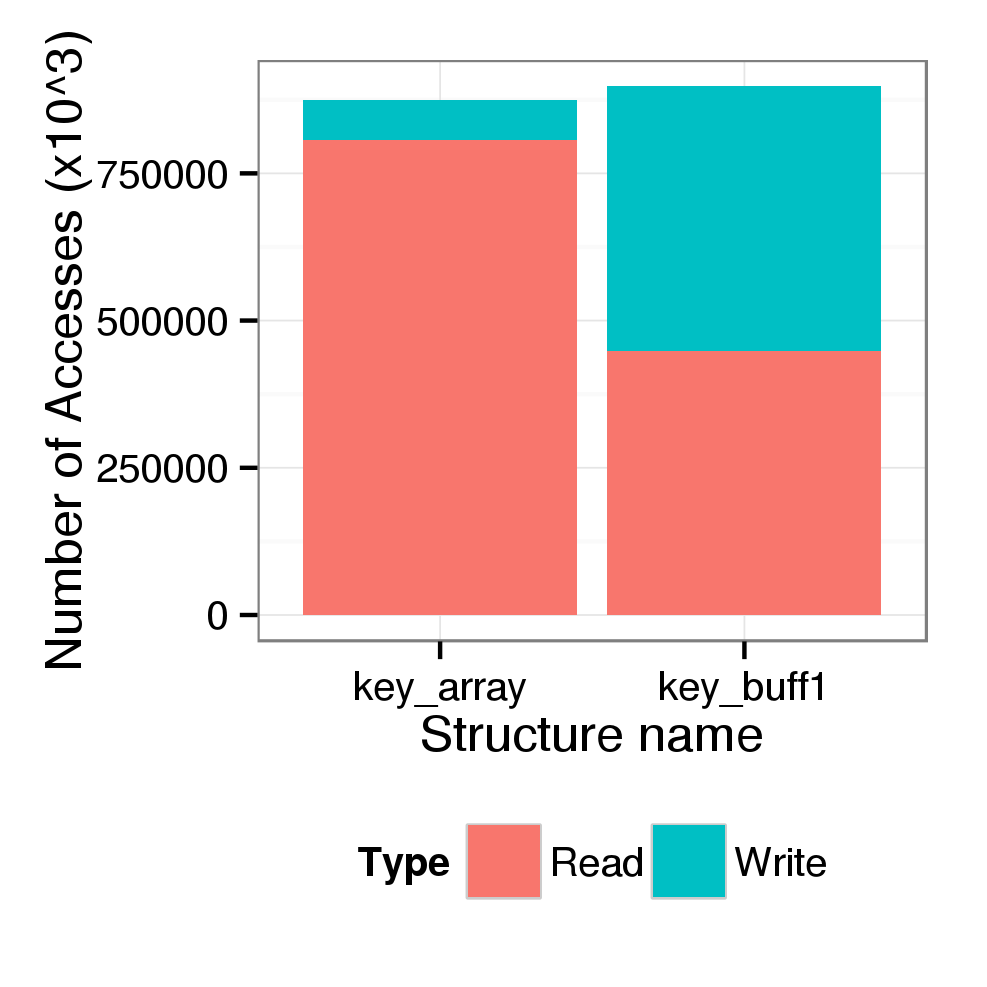
\includegraphics[height=.2\textheight]{example_rw}
        \label{fig:example_rw}
    }
    \subfigure[First touch distribution inside a structure.
    ]{
        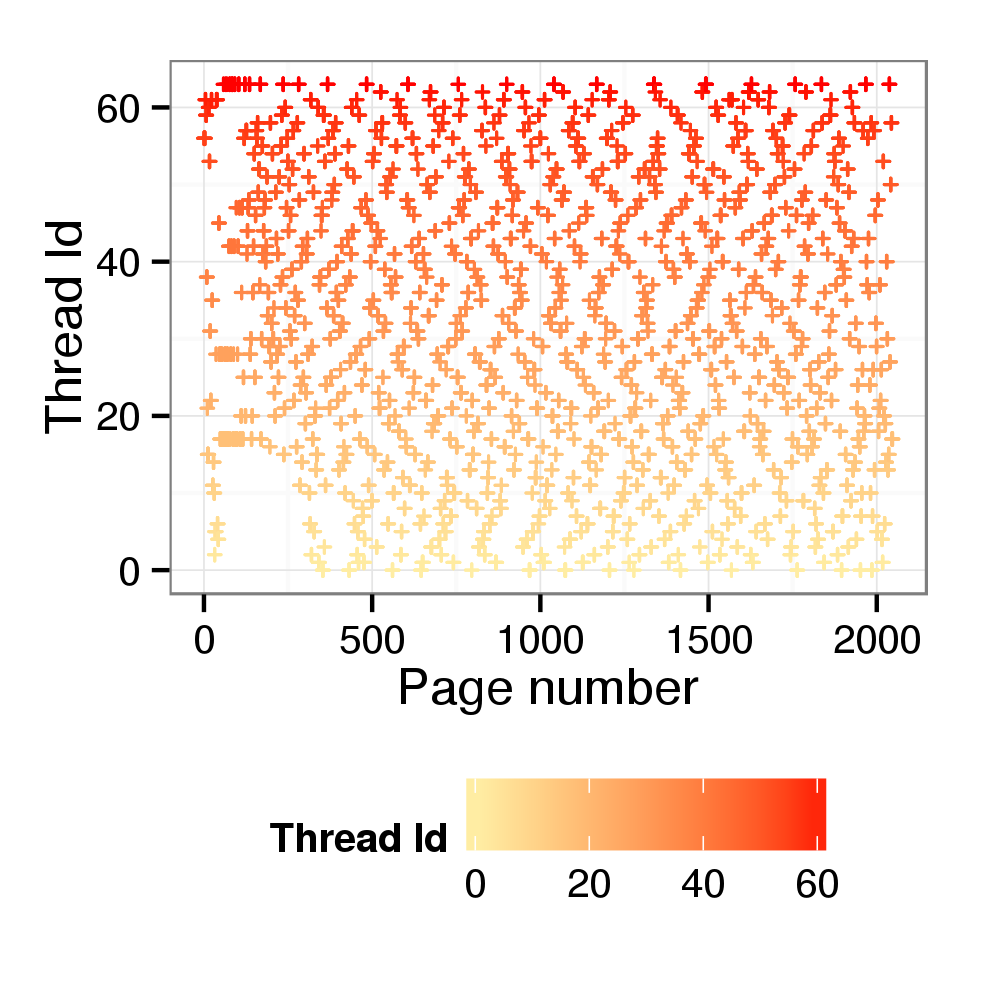
\includegraphics[height=.2\textheight]{example_ft}
        \label{fig:example_ft}
    }
    \caption{Example plots from \TABARNAC.}
    \label{fig:example_plot1}
\end{figure*}


After the introduction, the visualization focuses on the usage of data structures. Some
structures are not displayed for two reasons: either no accesses have been
detected during the analysis, which happens for structures used by external
libraries, or less than $0.01\%$ of the total accesses happens on them. This is
done to make the output more readable.
%However, it is possible to ask
%\TABARNAC not to ignore structures in the second case for a more detailed view.

The first series of plots presents information concerning the relative
importance of the data structures. It consists of two plots, showing first the
size of each data structure, as in Figure~\ref{fig:example_sz}, then the
number of reads and writes  in each structure (Figure~\ref{fig:example_rw}). These plots give a
general idea of the structures used by the parallel application.
Moreover, knowing the read/write behavior is very
useful as it determines the possible optimizations. For instance, structures
written only during initialization (or very rarely) can be relatively easily
duplicated, such that each NUMA node works on a local copy.

\begin{figure}[htb]
    \centering
    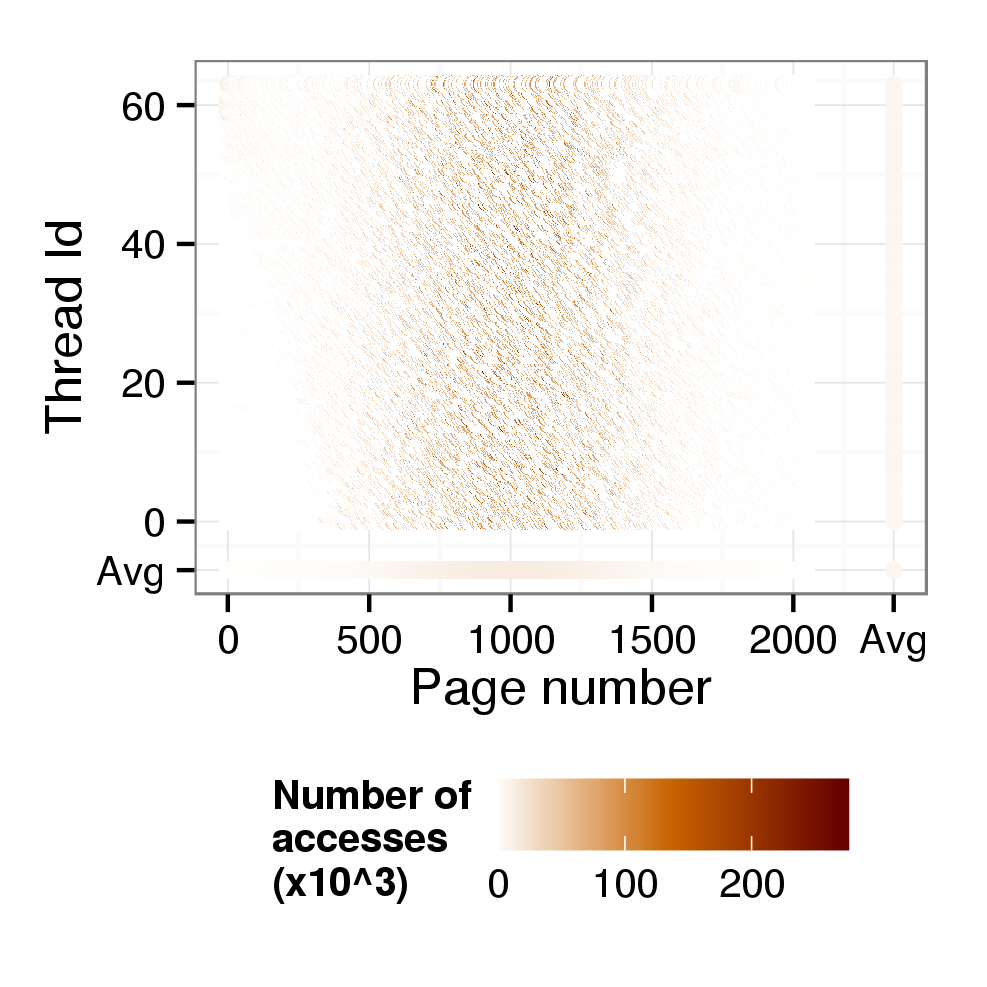
\includegraphics[height=.22\textheight]{example_dist}
    \caption{Per thread access distribution inside a structure.}
    \label{fig:example_dist}
\end{figure}

The second series of plots is the most important one. For each structure, it
shows for each page of each structure
which thread was responsible for the first touch
(Figure~\ref{fig:example_ft}). This information is important as the
default policy for \emph{Linux} and most other operating systems is to map a page as close as possible to the first
thread accessing it. If the first touch distribution does not fit the actual
access distribution, the default mapping done by \emph{Linux} might not be
efficient. To address this issue, the developer can either correct the first
touch or do some manual data mapping to ensure better memory access locality
during the execution.

Finally, \TABARNAC shows the density of accesses performed by each thread and
the global distribution. As we can see in Figure~\ref{fig:example_dist}, each
horizontal line represents the number of accesses on one page, there is one
line per thread and one for the average number of accesses. Moreover for each
thread the average number of accesses to the structure is displayed. The
darker is the line the more the thread accesses the page. It gives an easy way
to understand the data sharing between threads, the balance between pages and
threads. These plots can be used to identify inefficient memory usages and to
determine the best NUMA mapping policy.

